\chapter{Literature Study}
\label{chap:literature}

% TODO: write introductory text
\TODO{write introductory text}

\section{Multi-Criteria Decision Making (MCDM)}
\label{sec:mcdm}

Finding the right software package is often a daunting task. In order to suit the end-user's needs, the software should meet a large number of -- sometimes conflicting -- requirements and will result in making important trade-offs. Because of the these characteristics, software selection can be modeled as a Multiple-Criteria Decision Making (MCDM) problem \cite{Jadhav:2009, Jadhav:2011}.

There are two categories of MCDM problems: Multiple-Attribute Decision Making (MADM) problems and Multi-Objective Decision Making (MODM) problems. The first category involves sorting and ranking of a limited number of available alternatives, based on a number of decision criteria. In the latter category, there are no alternatives specified beforehand and the number of alternatives is effectively infinite \cite{Kahraman:2008}. 

The software selection process belongs to the category of MADM problems. Their goal is to find the best alternative in a set of alternatives and at the same to time create a ranking of all these available alternatives. % TODO: Reference!

There are a plethora of solution methods for the MADM problem. The following subsections will describe the most frequently used methods in literature, together with their advantages and disadvantages. 

% TODO: discuss cost vs benefit
\TODO{General remark for all methods: Separate costs from benefits, allowing to make a cost-benefit analysis afterwards. }

\subsection{Arbitrary scoring models} 
% TODO RFC: Is this a good naming?
\TODO{Question: Is this an appropriate name?}

There are a number of arbitrary scoring models but they all have one thing in common: for each criterion, the values are translated to a numerical score. In some cases, this score can be derived from the value of the criterion itself (e.g. speed, age, cost, \ldots). In other cases, a mapping is provided (e.g. in order to obtain a score $s$, at least features $f_1$, $f_2$ and $f_3$ should be supported).

Different methods are available to select potential candidates using these scores \cite{Kahraman:2008}:

\begin{itemize}
    \item When the ``dominance'' method is used, one alternative should clearly outperforms the other alternatives for at least one criterion. 
    \item When the ``maximin'' method is used, the final score of each alternative is equal to the lowest score of all criteria for this alternative.
    \item When the ``maximax'' method is used, the final score of each alternative is equal to the highest score of all criteria for this alternative.
    \item When the ``conjunctive'' method is used, an alternative should exceed certain thresholds for \emph{all} criteria.
    \item When the ``disjunctive'' method is used, an alternative should exceed certain thresholds for \emph{at least one} criterion. 
\end{itemize}

Additionally, the importance of the criteria can be accounted for by assigning weights. The final score can be calculated as the weighted sum, weighted product or weighted average.

The strength of these methods is that they are the most easy to use. However,  scores and weights are assigned arbitrarily and might get tough when there are a lot of criteria. Also, not all criteria are suitable for conversion into a numerical scale \cite{Jadhav:2009}.

\subsection{Analytic Hierarchy Process (AHP)}
\label{sec:ahp}

The Analytic Hierarchy Process (AHP) is ``a multi-criteria decision making approach in which factors are arranged in a hierarchic structure'' \cite{Saaty:1990}. It is developed by Thomas L. Saaty and is based on pairwise comparisons of both criteria and alternatives. 

The strengths of the AHP are that it (1) enables decision makers to structure a problem into a hierarchy, (2) that is provides a powerful tool for handling both quantitative and qualitative multi-criteria decision making problems and (3) that this system can deal with inconsistency \cite{Jadhav:2009}. 

The analytic hierarchy process consists of three stages. In the first stage, the factors that are important for the decision are organized into ``a hierarchic structure descending from an overall goal to criteria, subcriteria and alternatives in successive levels''. Organizing the factors in such structure helps the decision maker in getting an overview of the potentially complex relationships and also helps to assess the relative importance of the issues in each level. 

Structuring information in a tree is also backed by experiments of psychologist George Miller. He found that people can only deal with a few facts simultaneously; more precisely, seven plus or minus two \cite{Miller:1956}. 

In the second stage, the analytic hierarchy process establishes a ranking of the alternatives based on paired comparisons. 

\TODO{connect paragraphs}

Consider the case in which the relative comparison is derived from a given scale. For instance, where you have $n$ stones $A_1, \ldots, A_n$ with weights $w_1, \ldots, w_n$ respectively. 

\begin{gather}
    \begin{bmatrix}
        w_1/w_1 & w_1/w_2 & \ldots & w_1/w_n \\
        w_2/w_1 & w_2/w_2 & \ldots & w_2/w_n \\
        \vdots  & \vdots  &        & \vdots  \\
        w_n/w_1 & w_n/w_2 & \ldots & w_n/w_n    
    \end{bmatrix} % 
    \begin{bmatrix}
        w_1    \\
        w_2    \\
        \vdots \\
        w_n
    \end{bmatrix} = %
    n %
    \begin{bmatrix}
        w_1    \\
        w_2    \\
        \vdots \\
        w_n
    \end{bmatrix} \Longleftrightarrow %
    Aw = nw
    \label{eq:ahp}
\end{gather}

If $n$ is an eigenvalue of $A$, then $w$ is the corresponding eigenvector. The trace of a matrix, the sum of the elements on the main diagonal, is equal to the sum of its eigenvalues. Matrix $A$ has rank one because all rows of $A$ are linearly dependent on the first row and consequently, all eigenvalues except one are zero. Hence, $tr(A) = n$ and $n$ is the largest or pricipal eigenvalue of $A$.

\TODO{Prove validity of eigenvector method in AHP using \cite{Sekitani:1999, Saaty:2003}?}

\TODO{Add example}

The weakness of AHP is that it is a time consuming method due to the large number of pair-wise comparisons. Also, the ordering may change entirely when other alternatives are taken into account.

\subsection{Fuzzy MCDM}
\label{sec:fuzzy}

% TODO: Write section
\TODO{Write section}

Fuzzy logic was introduced in the mid `60s by Zadeh and was later applied to MCDM problems in the late `70s. Fuzzy logic allows to reason with imprecisely specified criteria like very high performance, low performance, etc. In classical approaches like those described above imprecision is dealt with first. When using the fuzzy approach, these imprecisions are only dealt with in the end, and only if necessary.

Fuzzy MCDM is based on three concepts \cite{FuzzySetApproach}:

\begin{enumerate}
    \item The set of alternatives is a \emph{fuzzy set}, i.e. the alternatives aren't precisely defined. The decision will thus be taken in a \emph{fuzzy environment}. 
    \item The decision is based on an aggregation of fuzzy preferences among alternatives.
    \item The decision is based on an evaluation of alternatives using a linguistic description.
\end{enumerate}

More concrete, let $A = \{a_1, \ldots, a_n\}$ be a finite set of given alternatives and let there be $m$ imprecisely defined criteria. Every alternative fulfills a criterion in a certain degree or does not fulfill it at all. In other words, for each criterion $G_j, j = 1, \ldots, m$ there is a set $G_j \subset A$ containing the alternatives fulfilling the criterion and the degree in which an alternative $a_i$ fulfills $G_j$ is expressed by the membership degree $G_j(a_i)$.

In order to decide the MCDM problem, constraints must be defined for each criterion. These constraints are specified as fuzzy sets as well meaning that a constraint $C_j$ is associated with a set $C_j \subset A$ containing the alternatives fulfilling $C_j$ in a certain degree. Again, a membership degree $C_j(a_i)$ is given.

Consequently, there are two fuzzy sets for every $j, j = 1, \ldots, m$, namely $G_j$ and $C_j$. The decision can now be obtained by composition and is given by the fuzzy set 
\begin{equation}
    D = (G_1 \alpha C_1) \beta \ldots \beta (G_m \alpha C_m)
\end{equation}
where $\alpha$ and $\beta$ are suitable fuzzy set operations. The alternative $a_k$ with the highest membership degree $D(a_k)$ is the best alternative.

\TODO{paraphrazed same source in previous three paragraphs, need a reference on each?}

\TODO{Add an example: For example, when buying a house these criteria could be \emph{nice neighbourhood}, \emph{great parking facilities}, \emph{reasonable price}, etc.}



\section{Software evaluation methodology}
\label{sec:selection_method}

Based on their literature review \cite{Jadhav:2009}, the authors have proposed a generic, six-stage methodology for the selection of software packages \cite{Jadhav:2011}.

\begin{enumerate}
    \item \textbf{Define selection criteria.} In the first stage, the evaluator defines the essential requirements for the software. If a certain software package does not meet a selection criterion, it is not a considered to be a suitable candidate and it should not be considered for further evaluation. 
    \item \textbf{Identify potential candidates.} During the next step, the evaluator searches for potential candidates. This step will result in a list of potential candidates.
    \item \textbf{List selected alternatives.} In this step, the evaluator will use the requirements from stage 1 to filter the list obtained from the previous stage. 
    \item \textbf{Define evaluation criteria.} In this stage, the evaluator has to define the evaluation criteria, arrange them in a hierarchy and define the value scales for each criterion. 
    \item \textbf{Evaluate selected alternatives.} During this phase, the evaluator will make a detailed comparison of the alternatives using the criteria obtained from the previous stage. A methodology like AHP can be used in this stage.
    \item \textbf{Select the most suitable alternative.} In this final step, all alternatives are ranked using the comparison results from the previous stage. Now, the best alternative can be chosen from the list of candidates. In general, a number of software packages will be taken into consideration and a selection will be made after additional steps (like for instance a cost-benefit analysis and/or contract negotiations with the vendor). 
\end{enumerate}

In the original paper \cite{Jadhav:2009}, the authors also suggest to include an additional evaluation stage after the selected packages has been implemented and integrated. During that stage, one should verify that the selected package does indeed meet the requirements.

\section{Mobile Architectures}

% TODO: talk about mobile hub
\TODO{Explain Mobile Hub/Mobile Orchestrator}

% TODO: discuss cost for each architecture
\TODO{discuss cost for each architecture}

There are already a number of paradigms for cross platform mobile application development \citep{Friese}. This section presents an overview of the available strategies by comparing different aspects: performance, look and feel, platform access, programming languages, development cost and distribution.

\subsection{Native App}

A native app is an application that is specifically designed to run on a particular platform. It is the default approach to develop applications for mobile devices. \fref{fig:native} shows an illustration of the overall architecture of such an app. 

\begin{figure}[h!]
    \begin{center}
        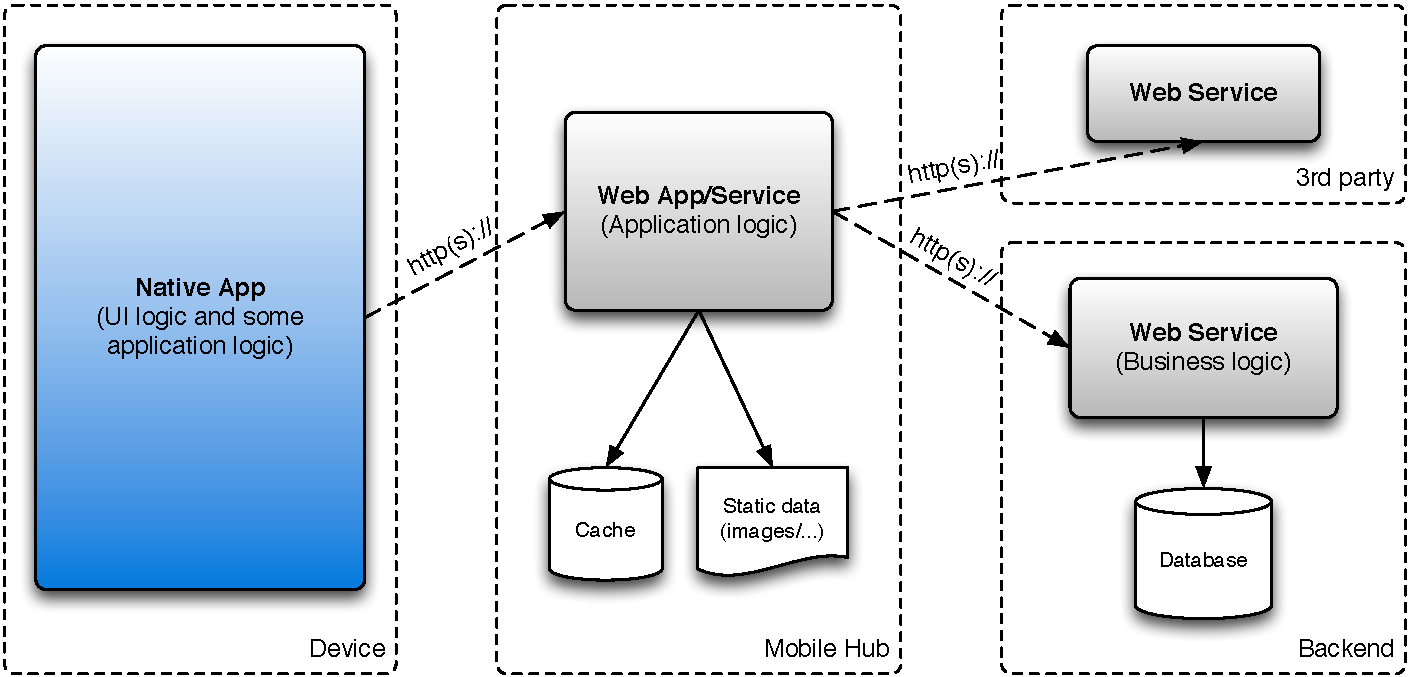
\includegraphics[width=\textwidth]{figs/native.pdf}
        \caption{
            Overall architecture of a native app. 
        }
        \label{fig:native}
    \end{center}
\end{figure}

Native apps are developed with the supplied SDK. Developers will need to get acquainted with the programming language used by said SDK but in return they will get full access to the platform and its features. As a result, the best performance can be obtained with this kind of app.

For the user interface, developers can use lots of interface elements such that they can present a familiar look and feel to the end user. 

Native apps can be easily distributed through an online marketplace like for instance the App Store or Google Play. 

Because native apps are designed to run on one platform only, this development strategy is not very well suited for cross platform development. If an application should run on multiple platforms, it has to be developed for each platform separately. This is costly.

\subsection{Web App}

Web apps are websites that are optimized for mobile browsers. Since every platform comes with a browser, this is the easiest way to get an application running on all platforms. An overview of the overall architecture for this kind of app is given in \fref{fig:web}.

\begin{figure}[h!]
    \begin{center}
        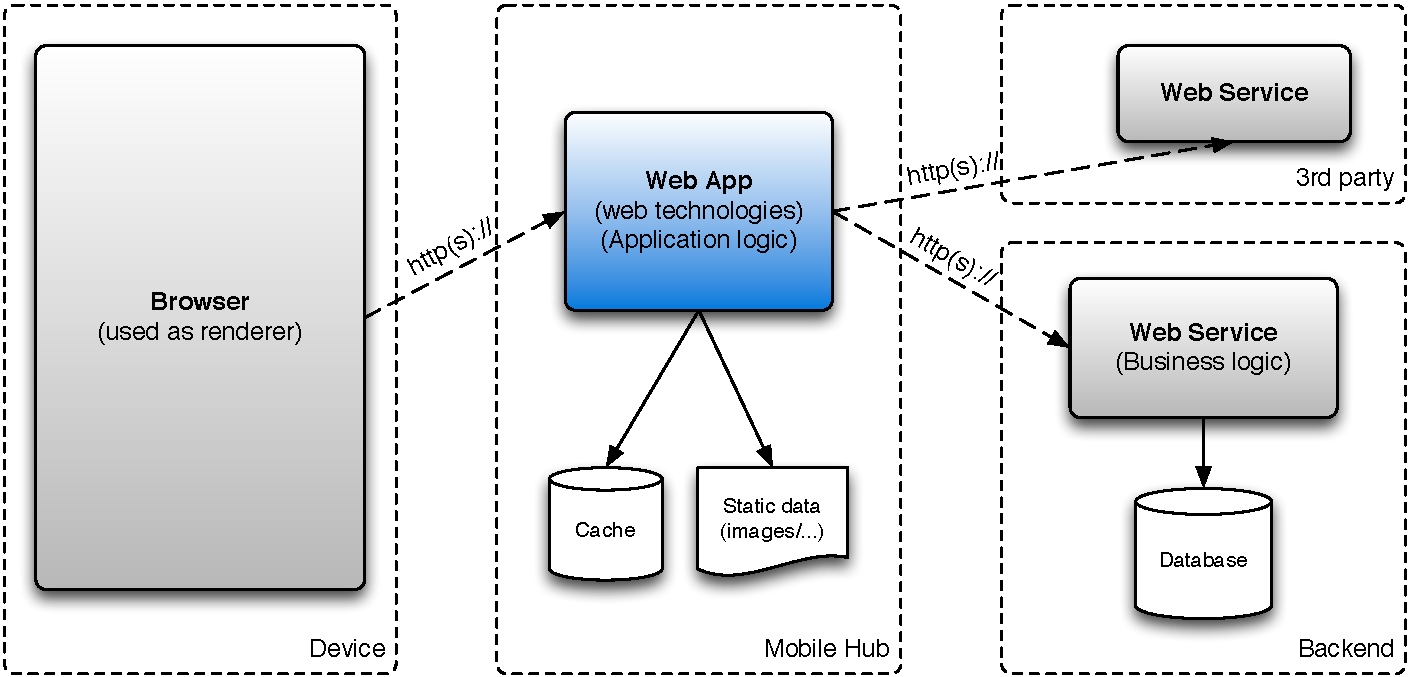
\includegraphics[width=\textwidth]{figs/web.pdf}
        \caption{
            Overall architecture of a web app.
        }
        \label{fig:web}
    \end{center}
\end{figure}

Web apps are not nearly as powerful as native apps. First of all, the application is not stored on the device. Web apps require an active internet connection which cannot always be guaranteed. Second, they are built with web technologies like HTML, CSS and JavaScript, which have to be interpreted by the browser at runtime. Third, web apps cannot access the system which means they cannot make use of the many unique features of a mobile device. 

With HTML5, web apps can get more powerful. They will be able to access device features, like the camera and other sensors \cite{MobileHTML5}. They will not even require an active internet connection because they can be cached on the device. However, HTML5 is still a draft and a lot of mobile browsers lack proper HTML5 support.

From a user interface perspective, web apps can be a problem as well. 
% TODO: complete paragraph
\TODO{complete paragraph}

Web apps are distributed easily: the only requirement is a valid URL. Web apps cannot be installed on the device though, but there are workarounds using Web Clips on iOS \cite{Safari:webclips} and bookmarks on Android. 

\subsection{Hybrid App}

Hybrid applications are the logical next step, combining native apps and web apps. The actual application is a web site, embedded in a web view, part of a native wrapper. The embedded website can access (parts of) the system through a bridge. An overview of the overall architecture is shown in \fref{fig:hybrid}. 

\begin{figure}[h!]
    \begin{center}
        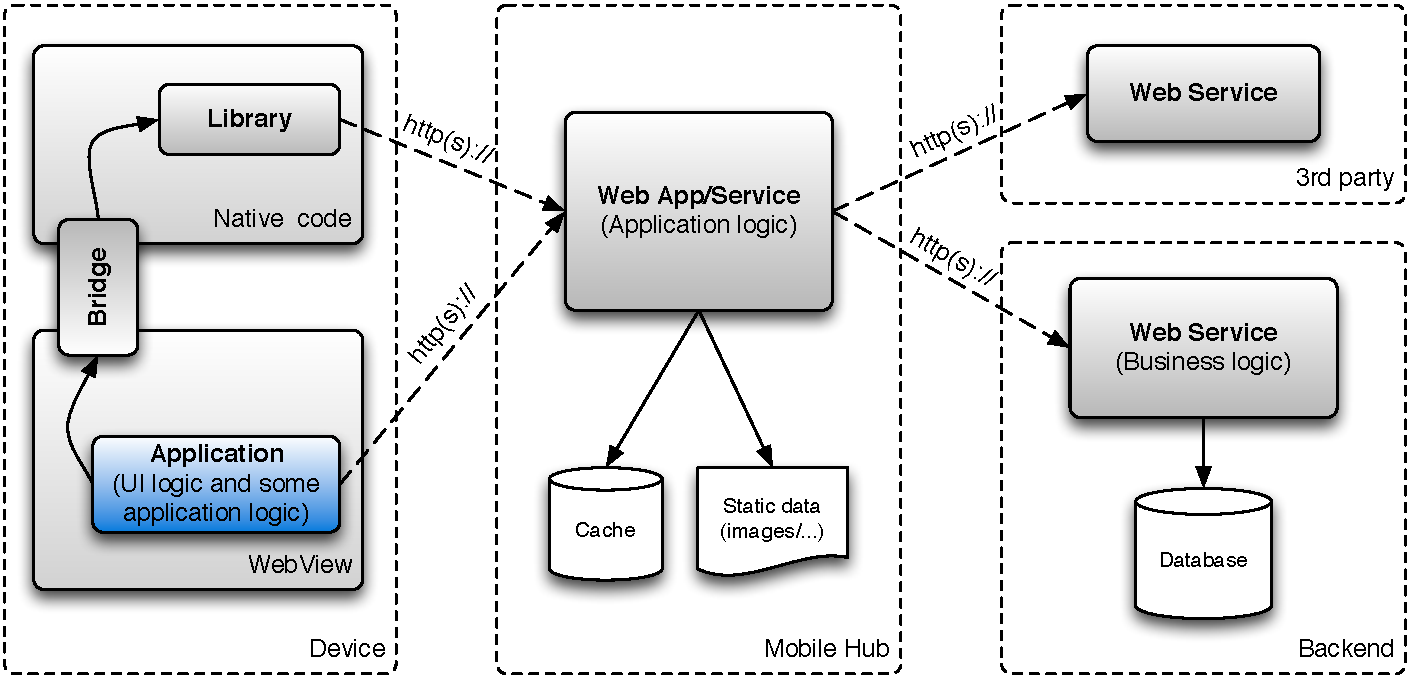
\includegraphics[width=\textwidth]{figs/hybrid.pdf}
        \caption{
            Overall architecture of a hybrid app.
        }
        \label{fig:hybrid}
    \end{center}
\end{figure}

Hybrid apps are part native app, part web app. Performance will be similar to web apps but some parts can be optimized by using native code. The websites inside the hybrid app are also much more powerful because they can access many device features that aren't available in HTML(5) through the bridge.

When it comes to the user interface, hybrid apps suffer from the same problem as web apps. 

Because hybrid apps are wrapped in a native container, they can be distributed just like native applications, through online marketplaces. 

\subsection{Interpreted App}

In an interpreted app, instructions in some language are translated to native instructions at runtime. \fref{fig:interpreted} shows the overall architecture of an interpreted app.

\begin{figure}[h!]
    \begin{center}
        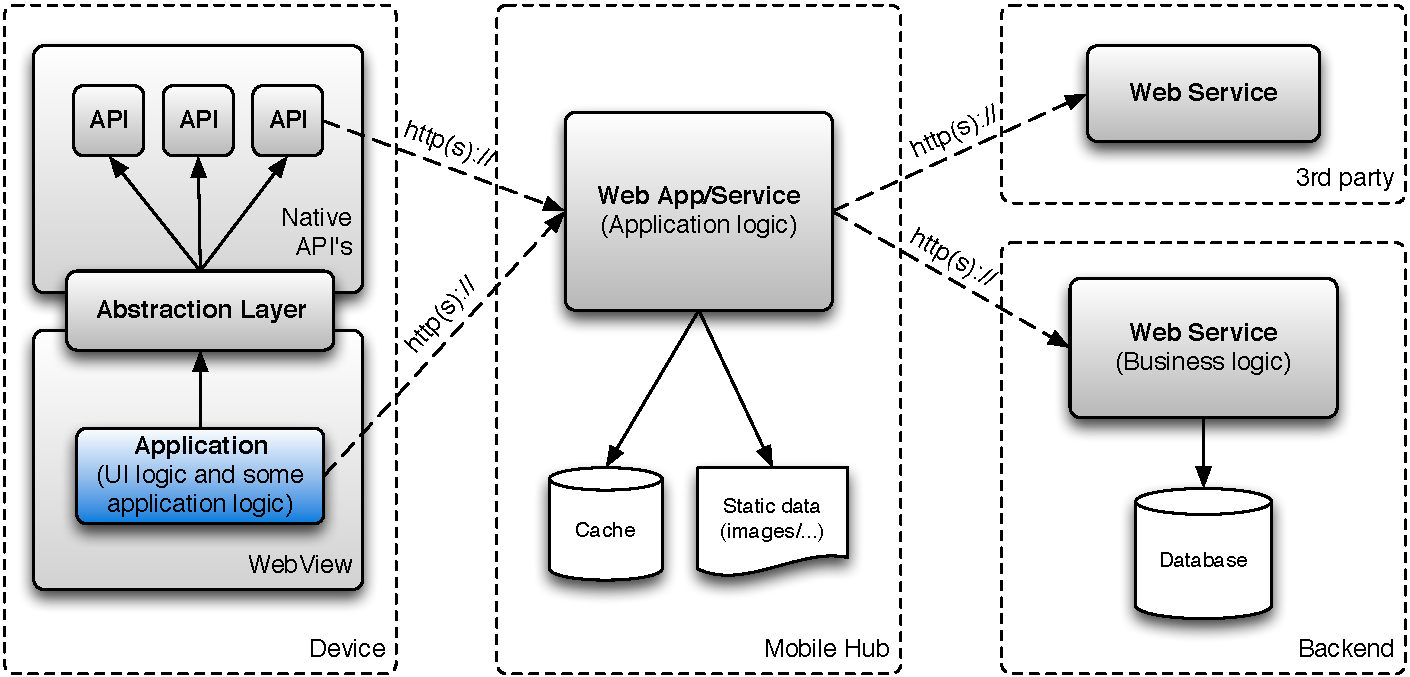
\includegraphics[width=\textwidth]{figs/interpreted.pdf}
        \caption{
            Overall architecture of an interpreted app.
        }
        \label{fig:interpreted}
    \end{center}
\end{figure}

Performance of interpreted apps depends on the interpreter and interpreted language but is better than web apps on average, though not as good as native apps. 

In an interpreted app, the user interface description is interpreted and rendered on the device using native interface elements. An interpreted app will have a familiar look and feel.

From the outside, interpreted apps -- just like hybrid apps -- look like native apps and can be distributed through online marketplaces.

\subsection{Cross Compiling}

Instead of translating instructions at runtime, one could translate instructions at compile time. The process is called cross compiling and the result is a truly native app. The overall architecture is sketched in \fref{fig:crosscompiled}. 

\begin{figure}[h!]
    \begin{center}
        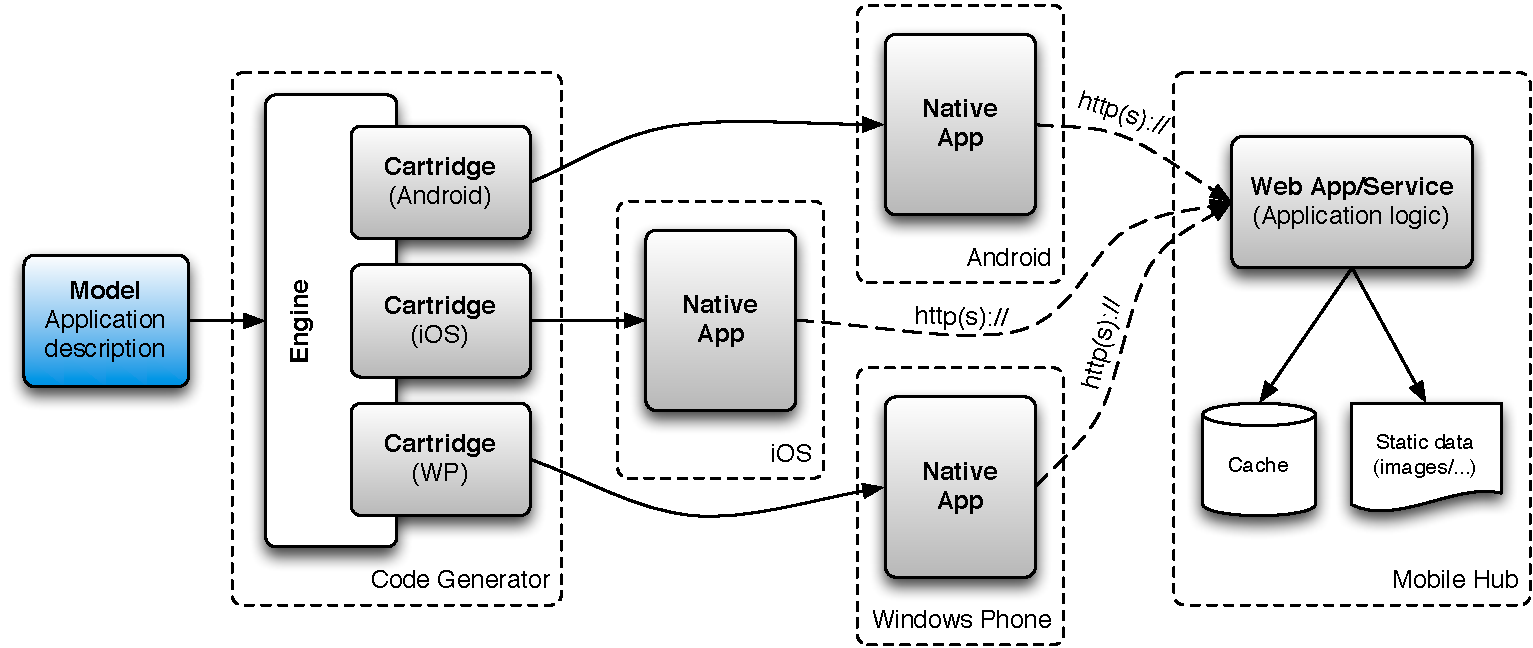
\includegraphics[width=\textwidth]{figs/crosscompiled.pdf}
        \caption{
            Overall architecture for cross compiled apps. 
        }
        \label{fig:crosscompiled}
    \end{center}
\end{figure} 

\subsection*{Summary}

\tref{tab:architectures} summarizes the results of the discussed strategies. It is important to note that there is no universal strategy that fits all use cases. A strategy must be chosen carefully, taking into account the client's wishes.

\begin{table}[h!]
    \begin{center}
        \begin{tabular}{l|c|c|c|c|c}
                             & Native      & Web                   & Hybrid      & Interpreted & Cross Compiled\\
            \hline
            Performance      & high        & low                   & rather low  & average     & high          \\
            Platform Access  & \checkmark  & $\times$ / \checkmark & \checkmark  & \checkmark  & \checkmark    \\
            Look \& Feel     & native      & non-native            & non-native  & native      & native        \\
            Distribution     & marketplace & URL                   & marketplace & marketplace & marketplace   \\
            Development cost & high        & rather low            & average     & average     & average       \\
        \end{tabular}
		\caption{
			Summary of cross platform mobile application development strategies.
		}
		\label{tab:architectures}
    \end{center}
\end{table}

\section*{Summary}